\scanpage{49}
\mspage{5)}
This operation of sums is the most trivial among the operations that
we shall have to make explicit and transcribe (combinatorially) in what follows.
Let us note at once, for given $(X,\widetilde\Sigma,R)$
\[
X\deleted{\unsure{\Sigma}}\text{ connected}\Longleftrightarrow
\Gamma\mathrm{MD}(X,\widetilde\Sigma,R)\text{ connected}
\]
more precisely
\[
\pi_0(X)\simeq\pi_0(\Gamma\mathrm{MD}(X,\widetilde\Sigma,R))
\]
\margin{give the formula for the genus of an
$\alpha\in\pi_0(X)\simeq\pi_0(\Gamma)$ in terms of the weighting ---
more generally the \uline{total genus} is
\[
g=\sum_{s\in S}g_s+c(\Gamma)
\]
\unsure{index of connectivity|order of connectivity} of the graph
$=\deleted{\unsure{\chi}}\mathrm{rg}\,H^1(\Gamma)$.}

\uline{Special cases.}

a) Case of $S_*\mathcal T^\pm_{\mathrm{top}}\
\deleted{\unsure{S_*\mathcal T_{\mathrm{top}}}}$
--- \unsure{that is|here} $\Sigma=\varnothing$, $\widetilde\Sigma=\partial X$.

This corresponds to the case of MD graphs \deleted{that} where
\inserted{all the edges are free, that is}
all the vertices are isolated (except for free edges)
\deleted{It} \inserted{The graph} is therefore determined by
\diagram{\begin{tikzcd}[ampersand replacement=\&,column sep=large]
A\ (\simeq\vec A=\vec A^\sigma)\arrow[r,"r"]\arrow[d]\&\mathbb N\\
S\arrow[r,"\gamma"]\&\mathbb N
\end{tikzcd}}

The case of $\mathcal T^\pm_{\mathrm{top}}$ corresponds to \unsure{choosing|setting} $\rho=0$,
so the situation is given by
\diagram{\begin{tikzcd}[ampersand replacement=\&]
A=A_0\arrow[d]\&\\
S\arrow[r,"\gamma"]\&\mathbb N.
\end{tikzcd}}

\margin{\figure{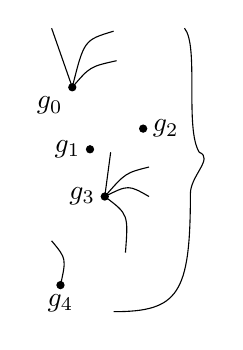
\begin{tikzpicture}[scale=.75]
\fill(0,0)circle(2pt);\node[below left]at(0,0){$g_0$};
\draw(0,0)--(-.35,1) (0,0)..controls(.2,.8)..(.7,.95)
(0,0)..controls(.3,.35)..(.75,.45);
\fill(.3,-1.05)circle(2pt);\node[left]at(.3,-1.05){$g_1$};
\fill(1.2,-.7)circle(2pt);\node[right]at(1.2,-.7){$g_2$};
\fill(.55,-1.85)circle(2pt);\node[left]at(.55,-1.85){$g_3$};
\draw(.55,-1.85)--(.65,-1.1)
(.55,-1.85)..controls(.9,-1.45)..(1.3,-1.35)
(.55,-1.85)..controls(.95,-1.65)..(1.3,-1.85)
(.55,-1.85)..controls(.95,-2.15)..(.9,-2.8);
\fill(-.2,-3.35)circle(2pt);\node[below]at(-.2,-3.35){$g_4$};
\draw(-.2,-3.35)..controls(-.1,-2.9)..(-.35,-2.6);
\draw(1.9,1)..controls(2.15,.7)and(1.9,-.7)..(2.15,-1.1)
..controls(2.4,-1.2)and(2,-1.5)..(2,-1.8)
..controls(2,-3.5)and(1.8,-3.8)..(.7,-3.8);
\end{tikzpicture}}}

The case of a connected \uline{structure}
$(\mathrm{card.}\,S=1\inserted{\text{ that is }S=\{s\}})$
\deleted{type $(g,\nu)$ of a}
is \deleted{\unsure{Determined}}\inserted{characterized}
by \deleted{\unsure{the genus}} the datum of the two integers $(g,\nu)$
$(g=\text{genus},\ \nu=\text{number of holes})$
\[
g=\gamma(s),\qquad \nu=\mathrm{Card}\,A.
\]
\mspage{48}
